\chapter{Konzeption}
\label{sec_konzeption}

\section{Offlinefähigkeit}
\label{sec_konzeption_offline}

Konventionelle Webanwendungen benötigen eine dauerhafte Verbindung zum einem Webserver, um Ressourcen abzufragen. Selbst bei kurzen Verbindungsabbrüchen ist eine Arbeit mit solchen Anwendung unmöglich und in vielen Szenarien nicht akzeptabel. In den folgenden Abschnitten \ref{subsec_konzept_caching-statische-ressourcen} und \ref{subsec_konzeption_caching-modell} werden Methoden beschrieben, um dieses Problem zu lösen und die Benutzererfahrung, durch Offlinefähigkeit einer Webanwendung, zu verbessern. 

Grundsätzlich kommen für das vorliegende Szenario zwei Varianten der Offlinefähigkeit in Frage. Die Variante \textbf{Überwindung von kurzen Verbindungsabbrüchen} sorgt dafür, dass die Anwendung trotz kurzfristiger Verbindungsabbrüche weiter reagiert. Die Anwendung kann die Verbindung beispielsweise wiederherstellen, jedoch kommt bei dieser Variante keine lokale Persistenz von Daten und Synchronisation mit dem Server zum Einsatz. 

Bei \textbf{\glqq{}echter\grqq{} Offlinefähigkeit} hingegen ist die Webanwendung auch ohne eine Internetverbindung funktionsfähig. Benutzer können nicht nur Daten anzeigen, sondern auch hinzufügen oder löschen. Dies wird durch eine lokale Zwischenspeicherung des benutzerspezifischen Anwendungsmodels (\glqq{}Application State\grqq{}) und dessen Synchronisation mit dem Applicationserver im Onlinezustand erreicht. Der Benutzer kann so kontinuierlich mit der Webanwendung arbeiten, ohne darauf achten zu müssen, ob er mit dem Internet verbunden ist oder nicht. \\
Zur Erfüllung der in Anforderung [FA-3] (vgl. Abschnitt \ref{sec_anforderungen_funktionale-anforderungen}) beschriebenen Offlinefähigkeit wird diese Variante bevorzugt.

\subsection{Caching statischer Ressourcen}
\label{subsec_konzept_caching-statische-ressourcen}

Während Webanwendungen einen Fehler anzeigen und eine weitere Verwendung unmöglich machen, sobald der Benutzer ohne aktive Internetverbindung versucht zu einer Seite zu navigieren, ist es in nativen Apps möglich sich weiter innerhalb der Anwendung zu bewegen. \\
Eine hybride Webanwendung muss also die Möglichkeit bieten, zu erkennen, ob eine aktive Internetverbindung vorhanden ist oder nicht und entsprechend darauf reagieren. Hier kommt die Service Worker API ins Spiel. Diese Technologie bietet Entwicklern die Möglichkeit einer optimalen Bereitstellung von Offline"=Benutzererfahrung.   

Wie in Abschnitt \ref{sec_grundladge_serviceworker} beschrieben handelt es sich beim Service Worker um eine Art Proxy zwischen der Webanwendung und dem Browser. Dadurch ist es möglich, Responses von HTTP-Request aufzunehmen, zu analysieren und ggf. anzupassen. Die Erkennung, ob ein Benutzer offline ist, ermöglicht es unterschiedlich auf einen HTTP"=Request zu reagieren. Dies ist eine Schlüsselfunktion, um die Anforderungen an Offlinefähigkeit erfüllen zu können.\\

\begin{table}[h]
\def\arraystretch{1.5}%  1 is the default, change whatever you need
\centering
\begin{tabularx}{\textwidth}{| l | X | }
    \hline
    \textbf{Bezeichnung} & \textbf{Beschreibung} \\
    \hline
    networkOnly & Ressourcen werden nur aus Netzwerk geholt \\
    \hline    
    cacheOnly & Ressourcen werden immer aus Cache geladen \\
    \hline
    fastest & Versucht von beiden Quellen zu laden und Antwortet mit schnellerem Response \\
    \hline
    networkFirst & Versucht zuerst aus dem Netzwerk zu laden und schaut in den Cache, wenn dies fehlschlägt \\
    \hline
    cacheFirst & Bezieht Ressourcen direkt aus dem Cache, fragt jedoch auch beim Netzwerk nach und aktualisiert bei Erfolg die Ressourcen im Cache \\
    \hline
\end{tabularx}
\caption{Übersicht Caching Strategien}
\label{tbl_konzeption_caching-strategien}
\end{table}

Tabelle \ref{tbl_konzeption_caching-strategien} zeigt die fünf grundsätzlich möglichen Strategien für das Caching von statischen Ressourcen, die mit Hilfe des Service Workers umgesetzt werden können. Damit die Benutzung der Anwendung auch ohne aktive Internetverbindung gewährleistet ist, müssen die Ressourcen ebenfalls bereitstehen, wenn das Gerät offline ist. Der HTTP"=Response muss also lokal gespeicherte Ressourcen ausliefern, wenn diese nicht über das Netzwerk bezogen werden können. \\

\begin{figure}[htp] \centering{
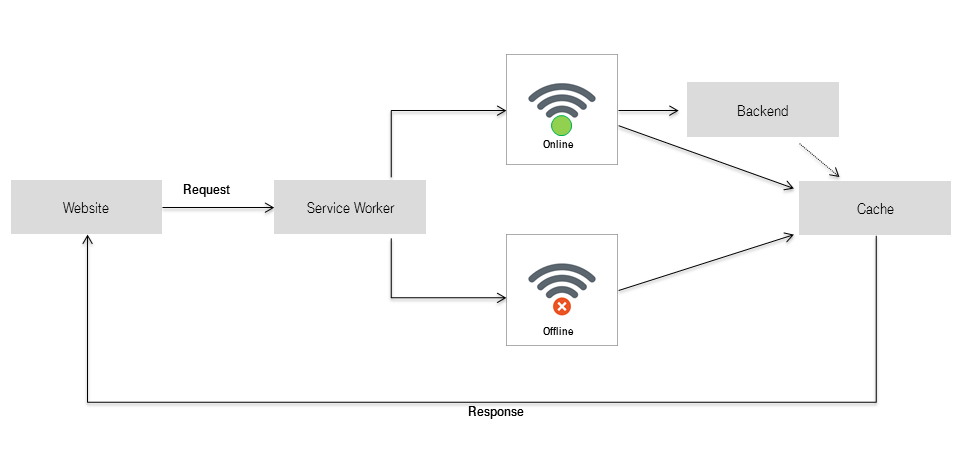
\includegraphics[width=0.9\textwidth]{images/konzept_cache.png}}
\caption{Caching Strategie \code{cacheFirst}}
\label{image_konzept_caching-strategie}
\end{figure} 

Das \code{cacheFirst}-Verfahren bietet sich für den vorliegenden Anwendungsfall an; die angeforderten Ressourcen werden direkt aus dem Cache geladen und anschließend versucht, diese im Hintergrund mit Ressourcen aus dem Internet zu aktualisieren (vgl. Abbildung \ref{image_konzept_caching-strategie}). Dadurch wird die Seite unabhängig vom Onlinezustand bei Anforderung schnell geladen und dem Benutzer eine optimale Offline-Benutzererfahrung ermöglicht.

\subsection{lokale peristente Speicherung und Synchronisation des Application State}
\label{subsec_konzeption_caching-modell}

Neben der in Abschnitt \ref{subsec_konzept_caching-statische-ressourcen} beschriebenen Vorhaltung der statischen Ressourcen muss die hybride Webanwendung ebenfalls einen Mechanismus zur Verfügung stellen, um das Datenmodell im Offlinebetrieb bereitzustellen.

\todo{Hier noch etwas über die Background.Sync API sagen\ldots}

\todo{Mehr Inhalt\ldots}

\newpage
\section{Web Push}
\label{subsubsec_konzeption_serviceworker_push-api}

Die Push"=API bietet Webanwendungen die Möglichkeit, von einem Server gesendete Nachrichten zu empfangen, unabhängig davon, ob die Webanwendung im Vordergrund oder sogar aktuell geladen ist. \\
Damit eine App, Push-Nachrichten empfangen kann, muss sie einen aktiven Service-Worker haben. Wenn der Service-Worker aktiv ist, kann er Push"=Benachrichtigungen über seinen internen Push"=Manager (\code{PushManager.subscribe()}) abonnieren.

Die resultierende \code{PushSubscription} enthält alle Informationen, die die Anwendung benötigt, um eine Push"=Nachricht zu senden. Neben einem Endpoint ebenfalls den für das Senden von Daten erforderlichen Verschlüsselungsschlüssel.

Der Service Worker wird nach Bedarf gestartet, um eingehende Push"=Nachrichten zu behandeln, die an den \code{ServiceWorkerGlobalScope.onpush()}- Eventhandler übergeben werden. Dies ermöglicht es Webanwendungen, auf empfangene Push"=Nachrichten, beispielsweise durch Anzeigen einer Benachrichtigung zu reagieren. \\
Für die Anzeige von Benachrichtigungen aus dem Service Worker heraus, wird laut Standard die Methode \code{ServiceWorkerRegistration.showNotification()} bereitgestellt.

Jedes Abonnement für einen Service Worker ist eindeutig. Der Endpoint für das Abonnement ist eine eindeutige URL. Die Kenntnis des Endpoints ist alles, was notwendig ist, um eine Nachricht an die Anwendung zu senden. Die Endpoint"=URL muss daher geheim gehalten werden, oder andere Anwendungen könnten Push"=Nachrichten an die Anwendung senden.

\subsection{Ablauf}

Abbildung \ref{image_konzeption_architektur-serviceworker-push} zeigt den grundsätzlichen Ablauf von Registrierung des Push"=Managers, über die Übertragung der Endpointinformationen bis hin zum Versand von Push"=Nachrichten. 

Zuerst  muss der Nutzer der Webanwendung auf eine Anforderung für Webbenachrichtigungen oder sonstige verwendete Berechtigungen reagieren, indem er die Berechtigungen erteilt (vgl. Abbildung \ref{image_konzeption_notification-permission}). \\

\begin{figure}[htp] \centering{
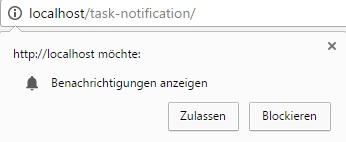
\includegraphics[width=0.5\textwidth]{images/notification_permission.jpg}}
\caption{Chrome - Berechtigungen zum Anzeigen von Benachrichtigungen}
\label{image_konzeption_notification-permission}
\end{figure} 

Nachdem die Berechtigung erfolgt ist, wird der Service Worker, lokal  für die Webanwendung registriert. 
Danach wird der Push"=Messaging"=Service, in unserem Fall \glqq Firebase Cloud Messaging\grqq{} (kurz FCM) mit der Funktion \code{PushManager.subscribe()} abonniert (vgl. Abbildung \ref{image_konzeption_architektur-serviceworker-push} Punkt 1). 

Mit Hilfe von \code{PushSubscription.endpoint} kann der mit der Subscription verknüpfte Endpoint abgerufen werden. Die Details werden an den Applicationserver gesendet, so dass er Push"=Nachrichten senden kann, wenn dies erforderlich ist (vgl. Abbildung \ref{image_konzeption_architektur-serviceworker-push} Punkt 2). Die Subscription-ID wird aus dem kompletten Endpoint entnommen. 

Auf Serverseite wird der Endpoint und alle erforderlichen Details, wie die Sender ID und Geräte ID in der Datenbank gespeichert, so dass sie verfügbar sind, wenn eine Push"=Nachricht an einen Benutzer bzw. ein Endgerät gesendet werden soll. \\

\begin{figure}[htp] \centering{
\centering
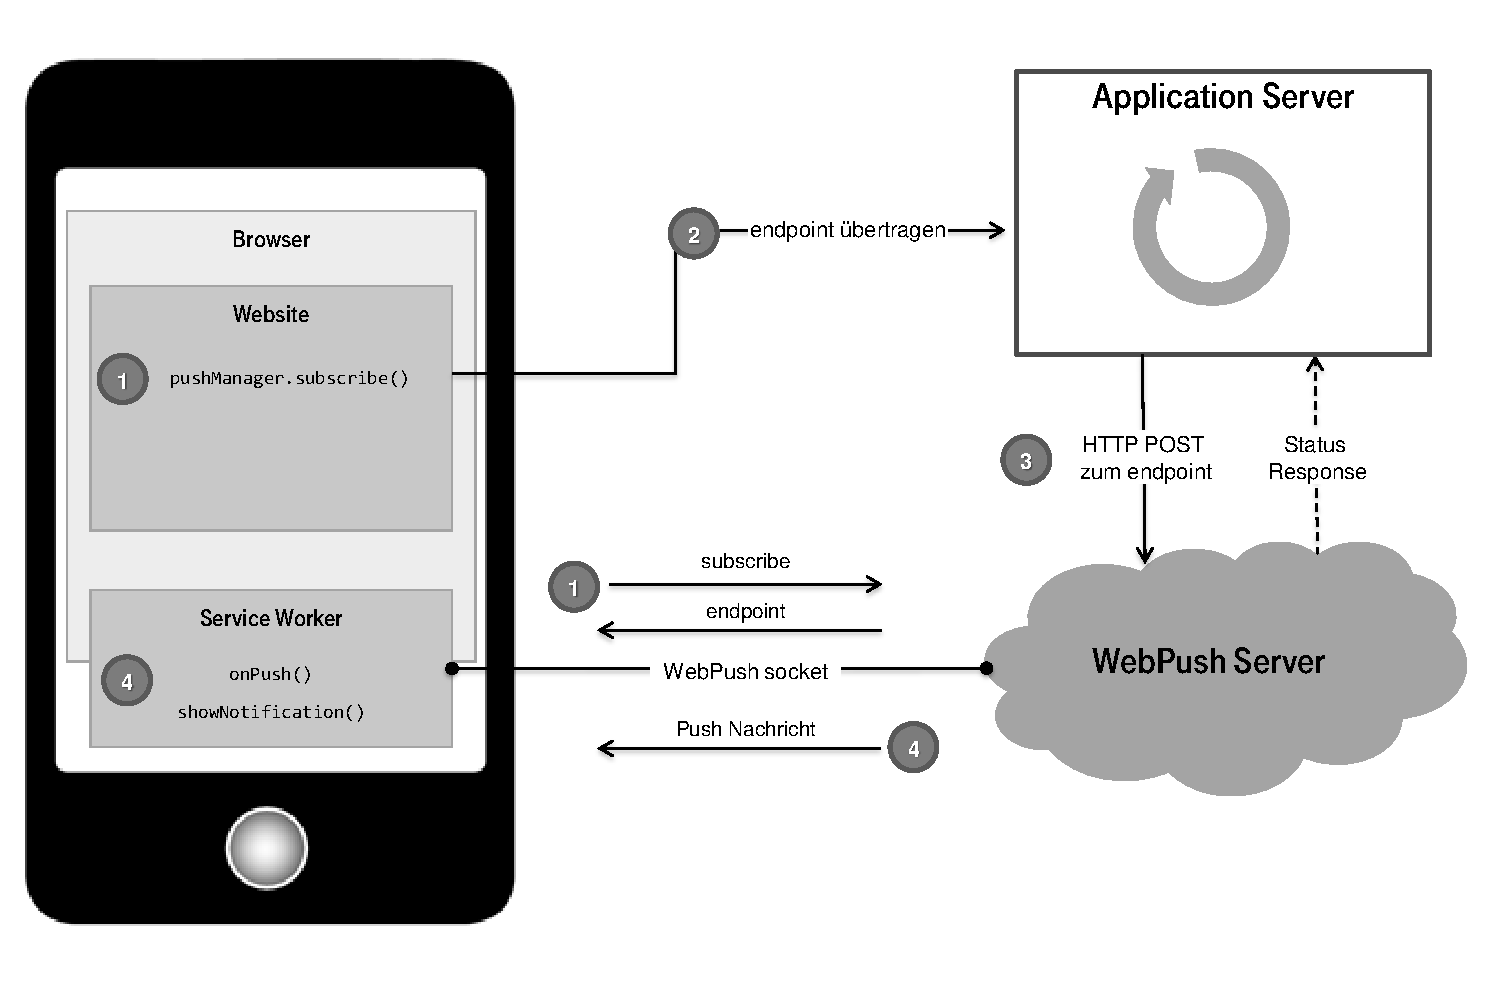
\includegraphics[width=0.9\textwidth]{images/architektur_serviceworker_push.pdf}}
\caption{Push mittels Serviceworker (in Anlehnung an MozillaWiki \cite{MOZ_WIKI})}
\quelle\url{https://wiki.mozilla.org/File:PushNotificationsHighLevel.png}
\label{image_konzeption_architektur-serviceworker-push}
\end{figure} 

Um eine Push"=Nachricht zu senden, muss ein HTTP-POST an die Endpoint"=URL (vgl. Abbildung \ref{image_konzeption_architektur-serviceworker-push} Punkt 3) gesendet werden. Die Anforderung muss einen TTL-Header enthalten, der begrenzt wie lange die Nachricht in der Warteschlange stehen soll, wenn der Benutzer nicht online ist.

Sobald die Push"=Nachricht vom Web Push Server erfolgreich versendet wurde, antwortet dieser mit einem Response, welcher eine eindeutige Message ID enthält. Diese referenziert auf eine bestimmte Push"=Benachrichtigung.

Den vom Applicationserver zuvor generierten Nutzdaten (Payload) wird diese Message ID zugeordnet und auf für Clientanfragen vorgehalten. \\
Sobald eine Push"=Nachricht vom Client empfangen wird, löst dies ein \code{onPush}"=Event aus (vgl. Abbildung \ref{image_konzeption_architektur-serviceworker-push} Punkt 4). Der Event-Listener reagiert mit einer direkten Anfrage beim Applicationserver und fragt ggf. vorhandenen Payload für die aktuelle Message ID ab.

\todo{Es ist auch so möglich: Besser ausformulieren}Um Nutzdaten in die Anfrage einzubinden, müssen diese verschlüsselt werden (mit dem öffentlichen Schlüssel des Clients (public key)).
Da wir uns gegen eine Nutzdatensendung über den Browserhersteller entschieden haben, entfällt bei uns dieser Schritt. 

\newpage
\section{Architekturbeschreibung}
\label{sec_konzeption_serviceworker_architektur}

Die Anwendung beruht auf dem Client"=Server"=Prinzip. Dabei stellt der Client lediglich die Oberfläche zur Interaktion mit dem Anwender dar. Außer der notwendigen UI"= und Serviceworker"=Logik ist die gesamte Geschäftslogik auf einen Business-Server (Applicationserver) ausgelagert. Die zentrale Datenbank sowie die statischen Ressourcen zur Darstellung des Client werden ebenfalls vom Applicationserver bereitgestellt. Für die Kommunikation steht eine RESTful"=Schnittstelle zur Verfügung.

\begin{figure}[htp] \centering{
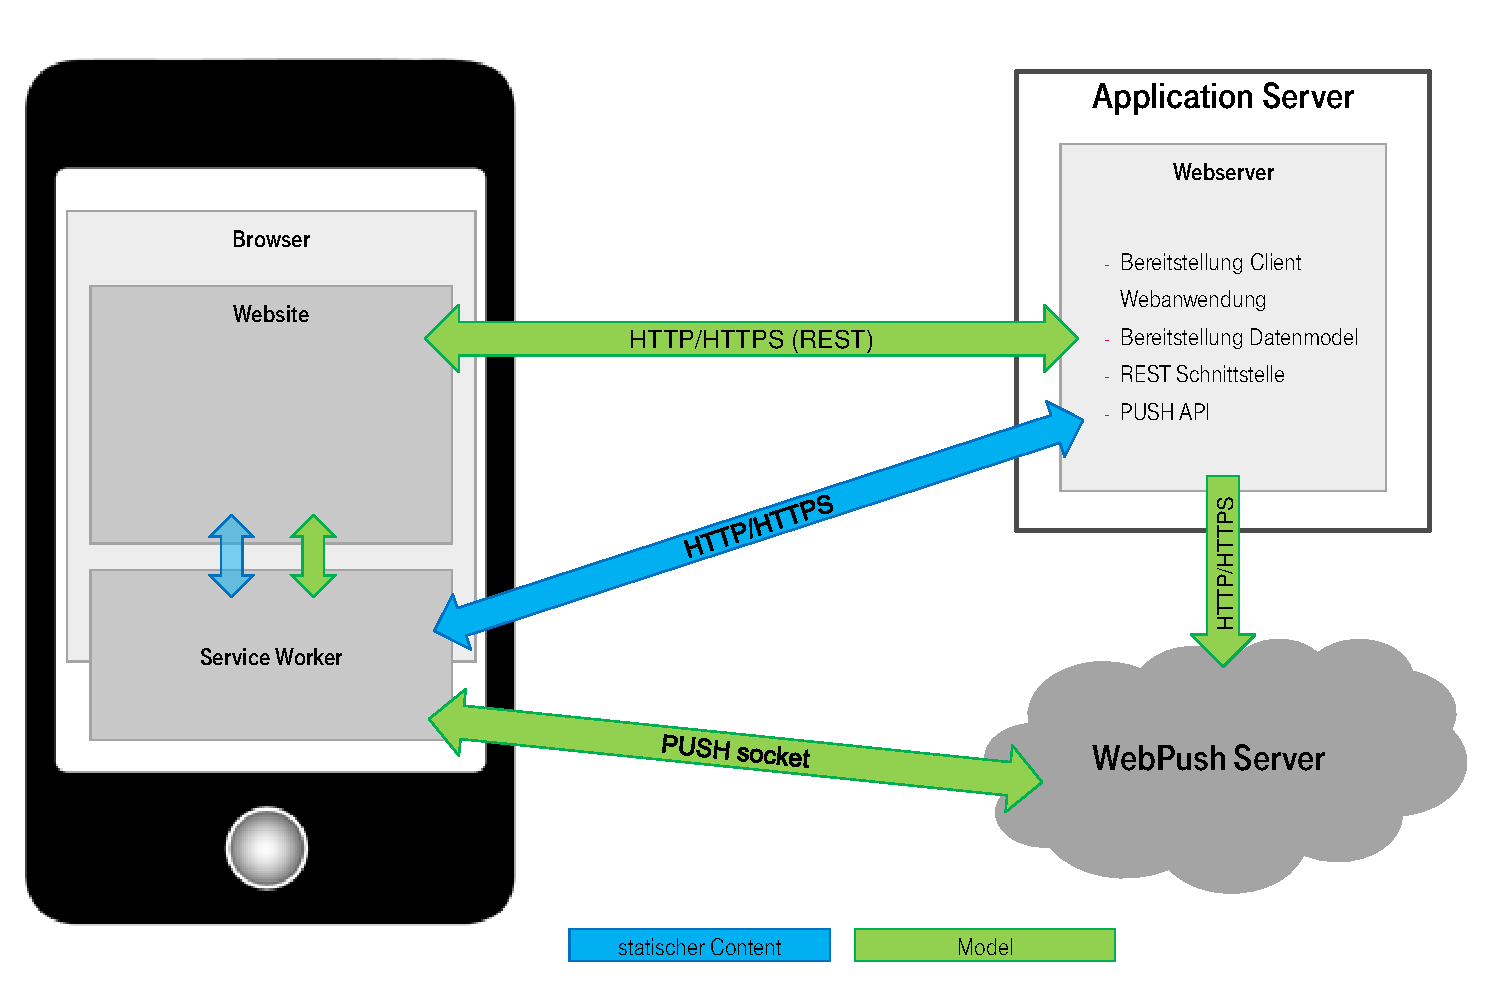
\includegraphics[width=0.9\textwidth]{images/architektur_serviceworker.pdf}}
\caption{Archtikturbeschreibung - Umsetzung mit Serviceworker}
\label{image_architektur-serviceworker-push}
\end{figure} 

\newpage
\section{Applicationserver}
\label{sec_konzeption_applicationserver}

Für die Bereitstellung der Geschäftslogik wird ein eigener Applicationserver benötigt. Als Plattform soll Node.js eingesetzt werden. Dadurch ist es mit überschaubarem Aufwand möglich, einfache Webanwendungen zu erstellen. Die Implementierung einer RESTful-Schnittstelle ist ebenso problemlos möglich wie die Anbindung von ORM-Tools für die Kommunikation mit einer Datenbank. 

\subsection{Datenbank}

Der Applicationserver stellt ebenfalls die Datenbank zur Verfügung und Verwaltet deren Zugriffe. Als Datenbank soll eine noSQL-Datenbank-Technologie verwendet werden. Diese ermöglicht eine objektorientierte Speicherung der Daten bei maximaler Flexibilität des Schemas. Node.js unterstützt die Anbindung sowohl von MongoDB als auch CouchDB. In der Implementierung wird MongoDB verwendet werden.

\subsection{REST-API}

Zur Bereitstellung von CRUD-Funktionalitäten über standardisierte HTTP-Methoden (vgl. Abschnitt \ref{sec_anforderungen_funktionale-anforderungen}, funktionale Anforderung [FA-4]) wird dem Applicationserver eine RESTful-Schnittstelle hinzugefügt. Eine Übersicht über mögliche API-Routen mit entsprechender HTTP-Methode ist in Tabelle \ref{tbl_konzeption_rest} dargestellt. 

\begin{table}[h]
\centering
\begin{tabular}{l | c | l }
    \textbf{Route} & \textbf{HTTP-Methode} & \textbf{Beschreibung} \\
    \hline\hline
    /api/signup & POST & Registriert einen neuen Benutzer \\
    /api/authenticate & POST & Authentifiziert einen Benutzer \\
    \hline
    /api/tasks & GET & Gibt alle Aufgaben zurück \\
    /api/tasks & POST & Legt eine neue Aufgabe an \\
    /api/tasks/:taskId & GET & Gibt eine einzelne Aufgabe zurück \\
    /api/tasks/:taskId & PUT & Aktualisiert eine einzelne Aufgabe \\
    /api/tasks/:taskId & DELETE & Löscht eine einzelne Aufgabe \\
    \hline
    /push/devices & GET & Gibt alle registrierten Geräte zurück \\
    /push/devices & POST & Registriert ein neues Gerät \\
    /push/payload/:messageId & GET & Gibt den Payload für MessageId zurück \\
\end{tabular}
\caption{Übersicht API Routen}
\label{tbl_konzeption_rest}
\end{table}

\subsubsection{Authentifizierung und Autorisierung} 

Für den Zugriff auf die CRUD-Methoden ist eine Benutzerauthentifizierung und Autorisierung notwendig. Registrierte Benutzer authentifizieren sich mittels Benutzername und Passwort über die Route \url{/api/authenticate} am Applicationserver. \\
Die notwendigen Parameter müssen im Request"=Body übertragen werden. Bei erfolgreicher Authentifizierung antwortet der Server mit einem Token innerhalb des Response"=Body. Allen weiteren Requests wird der Security"=Token als \code{Authorization}"=Header oder Body"=Parameter hinzugefügt. \\
Wird eine REST-Route ohne Authorization aufgerufen, antwortet der Server mit einem \code{HTTP 401}"=Response und signalisiert damit, dass eine Authentifizierung erforderlich ist. 

\section{Datenmodel}
\label{sec_konzeption_datamodel}

Die Umsetzung der Beispielanwendung benötigt kein komplexes Datenbankmodell. Abbildung \ref{image_konzeption_datenmodell} zeigt den Entwurf des Datenmodells. Dabei wurden nur notwendige Attribute dargestellt, um die Übersichtlichkeit in der Dokumentation gewährleisten zu können. \\

\begin{figure}[htp] \centering{
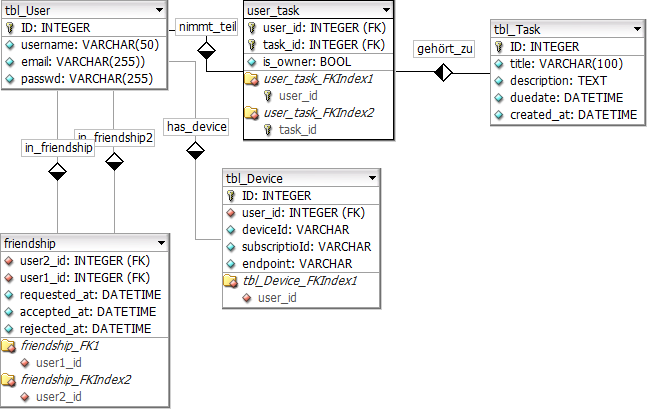
\includegraphics[width=0.9\textwidth]{images/model.png}}
\caption{Datenmodell}
\label{image_konzeption_datenmodell}
\end{figure} 

Zur Erfüllung der, in Abschnitt \ref{sec_anforderungen_nicht-funktionale-anforderungen} beschriebenen, nicht-funktionalen Anforderungen ist eine zentrale Benutzer-Entity notwendig. Diese enthält neben den notwendigen Anmeldeinformationen (Benutzername und Passwort) für jeden registrierten Benutzer eine E"=Mail Adresse. Diese wird beispielsweise benötigt, um die Registrierung zu bestätigen oder um ein vergessenes Passwort zurückzusetzten. 

Jeder Benutzer kann mehrere Aufgaben anlegen. Zu diesen Aufgaben können ein Titel, Beschreibung sowie ein Datum hinterlegt werden. Weiterhin können weitere Benutzer zu einer Aufgabe hinzugefügt werden. Dabei ist ein Benutzer immer \glqq{}Eigentümer\grqq{} während die anderen Benutzer als \glqq{}Teilnehmer\grqq{} agieren.

Zur Abbildung von Freundschaftsbeziehungen ist eine n:m-Beziehung zwischen User und User notwendig. Zu dieser Beziehung werden noch weitere Attribute wie \glqq{}Anfrage gestellt am\grqq{}, \glqq{}bestätigt am\grqq{} und \glqq{}abgelehnt am\grqq{} hinzugefügt.

Damit Benutzer unabhängig vom verwendeten Endgerät über Push"=Nachrichten benachrichtigt werden können, muss für einen Benutzer mindesten ein Gerät mit zugehöriger Push"=Subscription"=ID und Endpoint angelegt werden. Somit ist es möglich, einem Benutzer auf verschiedenen Endgeräten die gleichen Push"=Benachrichtigungen anzuzeigen.

\section{Client-Oberfläche}
\label{sec_konzeption_client-ui}

Um das \glqq{}Look \& Feel\grqq{} einer nativen Android"=Applikation zu erreichen wird nach Anforderung [NFA-1] (vgl. Abschnitt \ref{sec_anforderungen_nicht-funktionale-anforderungen}) das Framework \glqq JQuery"=Mobile\grqq{} verwendet.\\
Von Haus aus wird kein \glqq Material Design\grqq{} mitgeliefert. Das UI-Framework \textbf{nativeDroid2} setzt auf \glqq JQuery"=Mobile\grqq{} auf und bietet ein \glqq Material Design\grqq{}-Theme, sowie Hilfsklassen und Funktionen, die es erleichtern ein natives \glqq{}Look \& Feel\grqq{} in Webanwendungen zu gewährleisten. \\

\begin{figure}[htp] \centering{
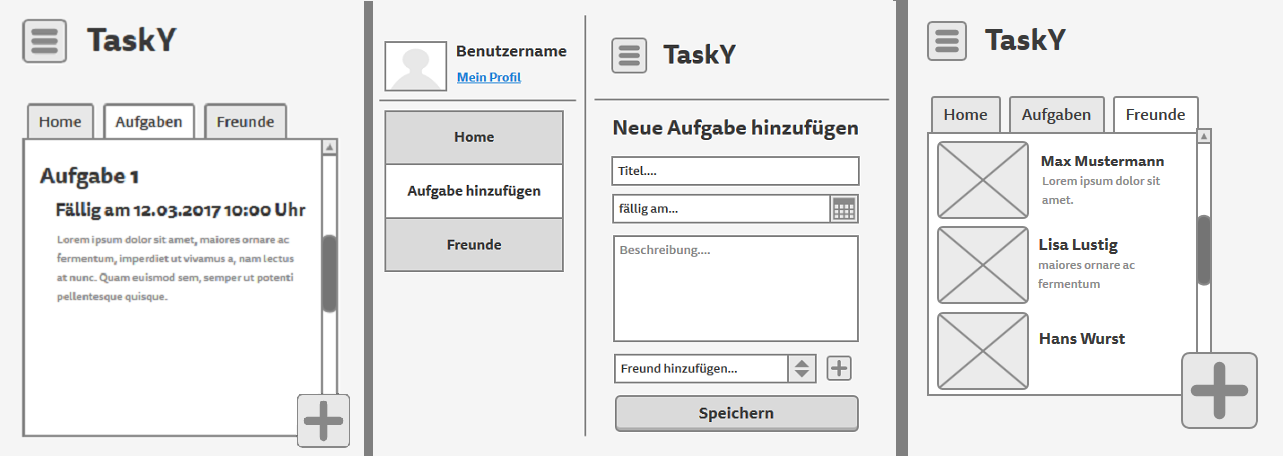
\includegraphics[width=0.9\textwidth]{images/mockup.png}}
\caption{Wireframe/Mockup"=Entwurf grafische Benutzeroberfläche}
\label{image_konzeption_gui}
\end{figure} 

Neben Ansichten für die Benutzerregistrierung und Anmeldung benötigt die Webseite Views für die Anzeige von Listen, eine Detailansicht für Listenelemente sowie ein Formular zum anlegen von neuen Aufgaben. 

Für die Navigation innerhalb der Webseite kommt eine vertikale Navigation zum Einsatz, die wie in nativen Applikationen ggf. ein"= bzw. ausgeblendet werden kann. Auf der Startseite ermöglicht eine horizontale Tab"=Navigation die Anzeige von verschiedenen Liste. Neben aktuellen Nachrichten wird eine Liste aller Aufgaben, sowie eine Kontaktliste integriert (vgl. Abbildung \ref{image_konzeption_gui}). 
